\documentclass[11pt]{ieeeconf}
\usepackage[margin=1in]{geometry}
\usepackage[english]{babel}
\usepackage[utf8x]{inputenc}
\usepackage{amsmath}
\usepackage{graphicx}
\usepackage{siunitx}
\usepackage{float}
\usepackage{url}
\usepackage{caption}
\usepackage{tocloft}
\usepackage{xcolor}
\usepackage{hyperref}
\usepackage{longtable}
\usepackage{csquotes}
\usepackage{listings}
\hypersetup{
  colorlinks = true,
  linkcolor = [rgb]{0,0,0.5},
  urlcolor = [rgb]{0,0,0.5}
}
\usepackage{lettrine}

\graphicspath{ {./images/} }
\renewcommand\cftaftertoctitle{\par\noindent\hrulefill\par\vskip-0.5em}

\newcommand\blfootnote[1]{%
  \begingroup
  \renewcommand\thefootnote{}\footnote{#1}%
  \addtocounter{footnote}{-1}%
  \endgroup
}

\title{Breast Cancer Cellularity Prediction from H\&E Images Challenge}
\author{Raj Patel, Blaze Kotsenburg}

\begin{document}
\begin{titlepage}
  \newcommand{\HRule}{\rule{\linewidth}{0.5mm}} % Defines a new command for the horizontal lines, change thickness here
  
  \vspace*{\fill}
  \center % Center everything on the page
  
  { \huge \bfseries Breast Cancer Cellularity Prediction from H\&E Images Challenge}\\
  \HRule \\[1cm]

  \large Raj Patel\\
  \large Blaze Kotsenburg\\[1.5cm]

  \normalsize ECE 6960 - Deep Learning for Image Analysis\\
  \normalsize \today\\[4cm]
  
  \vspace*{\fill}
\end{titlepage}

\maketitle
\begin{abstract}
Breast cancer affects about 1 in 8 women in the United States alone \cite{web1}. Being able to identify breast cancer in its early stages is of the utmost importance. Deep learning can be used to detect breast cancer from whole slide images of breast cancer hematoxylin and eosin stained pathological slides with high accuracies. This can save human labor and help detect breast cancer in its early stages, preventing it from spreading to neighboring cells. This research paper focuses on applying multiple convolutional neural network (CNNs) models to whole slide images of breast cancer to increase prediction accuracy of cancer cell detection.
\end{abstract}

\begin{keywords}
  Convolutional Neural Network (CNN), Deep Learning, ResNet
\end{keywords}

\blfootnote{This paper was submited for review on \today.}
\blfootnote{R. Patel is with the Department of Computer Engineering at the University of Utah, Salt Lake City, UT 84101 USA (e-mail: raj.patel@utah.edu).}
\blfootnote{B. Kotsenburg is with the Department of Computer Engineering at the University of Utah, Salt Lake City, UT 84101 USA (e-mail: bkotsenburg@gmail.com).}

\section{Introduction}
\lettrine{B}{reast} cancer remains one the most commonly diagnosed cancers in women, apart from skin cancers \cite{carol}. It was estimated that in 2013 there would be approximately 232,340 new cases of invasive breast cancer and 39,620 breast cancer deaths in US women alone \cite{carol}. Recorded cases of breast cancer and mortality rates are expected to continue to increase in the future. Because of these statistics, breast cancer research remains a top priority for research in the biomedical field due to its prevalence in women.

Current methods used to detect breast cancer consist of breast exams, mammograms, breast ultrasounds, biopsy of breast cells, or magnetic resonance imaging (MRI) \cite{web2}. Breast exams require a doctor to examine lymph nodes near the armpit region to detect any abnormalities. Exams are generally the first step in the screening process. If any abnormalities are found, further screening will be needed. Mammograms take x-rays of the breast, producing a visualization of  any abnormalities that may be present in deeper tissue. Ultrasounds create a similar screening to x-rays. Ultrasounds can detect lumps and determine whether they are solid mass or a filled with fluid (cyst). Biopsies, which are probably the most promising test, take core tissue samples from suspicious areas. The tissue samples are sent off to a laboratory to be tested and examined by experts. Biopsies also allow for experts to determine the type of cell present in the tissue sample, which is beneficial for diagnosis. Finally, MRI’s are used to produce images from magnet and radiowaves. Images are then observed by a radiologist to determine if any anomalies exist in the breast \cite{web2}.

All of the above methods are used to attempt to detect breast cancer in its earliest stage possible. Excluding biopsies, most of these methods are not going to detect breast cancer in its early cellular stages. Deep learning can be extremely beneficial in breast cancer detection in the early development stages of the cancer cells. Biopsies provide tissue samples that can be imaged as whole slide images (WSIs). Convolutional neural networks (CNNs) can be applied to these images to generate a prediction for the presence of breast cancer in the image and even predict the type of cancer.

We found this topic to be interesting because it is within a field that has an extremely high priority of research. The priority is so high because of how high the mortality rates are and how prevalent these cancers are in woman. SPIE Medical Imaging is an organization where the latest information on medical data is presented. In 2018, SPIE released a challenge to detect breast cancer called BreastPathQ \cite{spie}. In this challenge, patient image samples were provided for participants of the challenge to give a probability prediction on the presence of breast cancer in the image.

The sections below will discuss a literature survey, discussing models that have already been applied to breast cancer detection; the materials and methods used during our own experimentation and research; followed by the results produced from our models; and a conclusion section discussing what we found to work best for our models.

\section{Literature Survey}
Deep learning is continuing to be integrated into the field of breast cancer detection. A multitude of research papers use CNNs to make predictions for the presence of breast cancer cells from WSIs. In our research on the topic, we found research papers that used a wide variety of CNNs to aid in breast cancer detection. In the following paragraphs, we will discuss a few of the models we discovered and found to be interesting. Some of these models influenced the implementation of our own models.

\subsection{CycleGAN}
One model that we found particularly interesting was a variation of a generative adversarial network (GAN). The model was named CycleGAN by the researchers who implemented the model. CycleGAN is based on domain adaptation using a cycle consistent generative adversarial network, which is where its name comes from \cite{wollmann}. Domain adaptation is needed when a model is used to make predictions on data from different (but related) targets of distribution \cite{web3}. An example of this is spam email detection. A model must adapt to different users who may have a different variation of emails that they receive \cite{web3}. The CycleGAN model uses model averaging for boosting in order to generate classification results. The results determine a slide level class and are further combined to make a patient level prediction \cite{wollmann}.

The CycleGAN model uses end-to-end learning and only requires slide level annotations. Other models are based on pixel level annotations for training, which is what differentiates the CycleGAN model from previous models. The model is also combined with a densely connected deep neural network (DenseNet). “The CycleGAN enables unpaired domain adaptation to transfer the appearance of data from one source to another source (e.g., different medical centers) in an unsupervised manner” \cite{wollmann}. The model was used on the CAMELYON17 challenge dataset, showing that domain adaptation improves classification results even compared to high performing data augmentation.

This model offers faster computation times and can be completely automated for patient level breast cancer detection. The average time that this model takes to generate a classification for a 512x512 image is 0.04 seconds and has a total computation time of 0.78 seconds on a WSI \cite{wollmann}. This totals to 3.9 seconds to generate a prediction for a patient level grade. Improvements were made on this models forward pass, which proved to be ten times faster than the original DenseNet. The model is unsupervised and can be used between different medical centers because of the domain adaptation \cite{wollmann}.

\subsection{Inception and ResNet}
Inception and ResNet models were used in another research paper we discovered. Data augmentation was applied to the data set for both models. Data was resized, flipped, rotated, and cropped \cite{hamidreza}. Data augmentation enabled the models to be invariant to different types of images shown from different datasets. Color distortion was also performed on the images which altered the hue, brightness, saturation, and the contrast of the images. During evaluation however, the images were normalized and re-sized to specific widths and heights \cite{hamidreza}.

In the study, the researchers tested and examined several Inception and ResNet frameworks. Inception V1, V2, V3, and V4 were used along with ResNet V1 50, V1 101, and V1 152 frameworks \cite{hamidreza}. Weights for the networks used the pretrained weights from ImageNet Inception and ResNet pretrained models. During the study, they used transfer learning to train the final layers of the models while retaining the pretrained weights.

\begin{figure*}[tb]
  \centering
  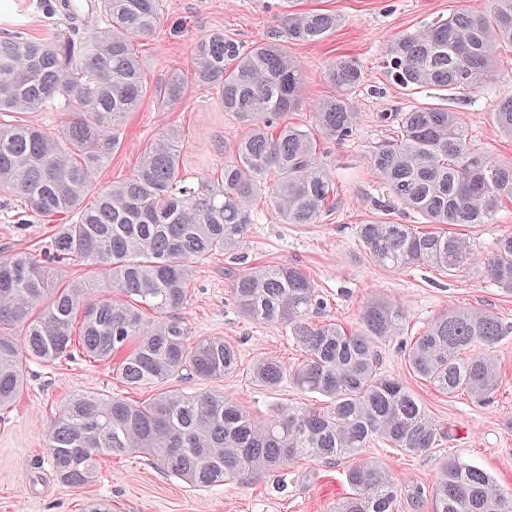
\includegraphics[width=14em]{99791_1.png}
  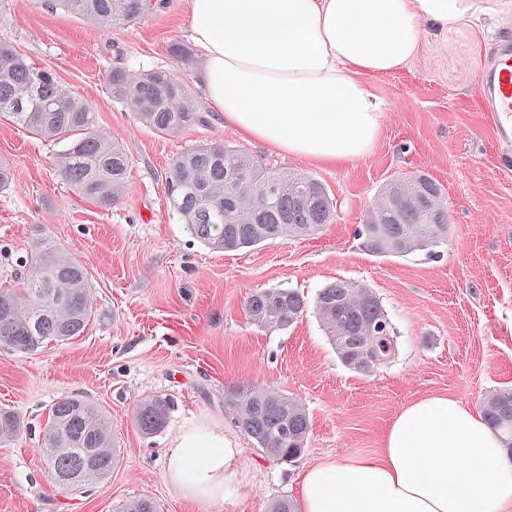
\includegraphics[width=14em]{99791_16.png}
  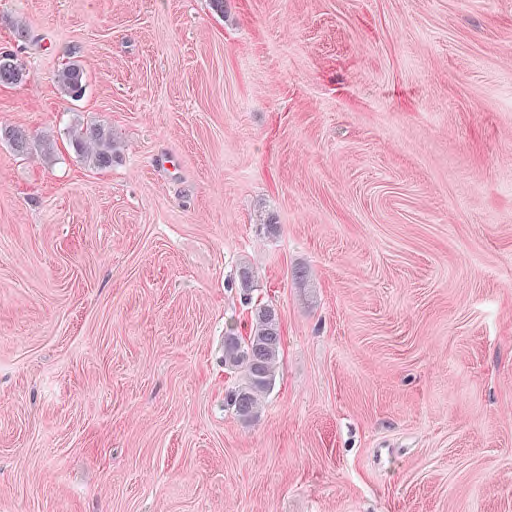
\includegraphics[width=14em]{99791_29.png}
  \caption{BreastPathQ patient image samples \cite{spie}.}
  \label{fig:samples}
\end{figure*}

The architecture for the Inception model was implemented with a 1x1 factorized convolutional layer; a rectified linear unit (ReLU); a 3x3 convolutional layer; an auxiliary layer with the combination of logits and average pooling;  a 1x1 convolution layer;  followed by a fully connected layer; and ending with a softmax activation layer \cite{hamidreza}. The ResNet model used residual connections between deep and shallow layers to adjust and control the error rate \cite{hamidreza}.

Both models showed extremely promising results with high classification accuracies. The Inception V1 model produced a classification accuracy of 91.7\%. The ResNet V1 50, 101, and 152 produced classification accuracies of 99.8\%, 99.6\%, and 99.6\% respectively. It appears that deeply layered ResNets can improve classification accuracies by a tremendous amount.


\section{Materials and Methods}
\subsection{Dataset}
The BreastPathQ dataset included an evaluation metric which was a great help in this project. The challenge provided us with training, validation, and test datasets. The training dataset contained 2,579 images while the validation set contained 185 images. Few of the training images can be visualized in Fig. \ref{fig:samples}. Originally we planned on predicting on the test dataset and uploading the result to the Spie Challenge website. However, the website was unresponsive during our testing. To compensate, we used three patient’s data samples, which was roughly 120 images, for testing. The following is the metric provided from the Spie Challenge:

\begin{displayquote}
``The prediction probability will be calculated for each method for each reference standard (pathologist 1 and pathologist 2), then averaged to determine a final overall prediction probability value. If the prediction probability values across multiple methods are the same (a tie), the prediction probability value for the subset of cases with mean reference values below 50\% will be used as a tie breaking subset of cases. The same approach described above will be used to estimate a prediction probability value for this subset of cases. If the methods are still tied in performance, a coin flip will be used to determine a winner.

The definition of prediction probability that is used is the following:

$$p_k=\frac{\frac{P - Q}{P + Q + T} + 1}{2}$$

where P is the number of concordant pairs, Q the number of discordant pairs, and T the number of ties only in the submitted labels.''\cite{spie}
\end{displayquote}

\subsection{Framework}
Throughout our project, we used Python version 3.6 coding language. To represent all of our deep learning networks, we used the PyTorch library. We created our own BreastPathQ dataset class by inheriting PyTorch’s DataSet class. This class parsed all of the images and mapped it to its patient ID. To save memory, the image is only loaded on demand.

Running our code is fairly straightforward. Our program takes in three command line arguments. First argument is for the machine type. We need this argument to develop on our local machine since our local environment had less GPU memory than the CADE machines. Second argument is to select which CNN model to train. There are three possible choices for our CNN model: ‘resnet’ for ResNet, ‘simple’ for our initial ConvNet, and ‘improved’ for our improved ConvNet. Finally, the last argument is for the optimizer. There are two options for the optimizer ‘adam’ and ‘sgd’ (SGD + Momentum). A command to run the improved model with SGD + Momentum running on CADE would look as following:

\begin{lstlisting}
python3.6 main.py cade improved sgd
\end{lstlisting}

\subsection{ResNet}
While reviewing research papers based on breast cancer cell detection via deep learning, we found a handful of papers that used deep ResNet models. Most of the successful models that we reviewed achieved accuracies of up to 99.8\% with models deeper than 50 layers. With our resources, we weren’t able to implement a model as deep as the ones reviewed since we have constraints on our RAM and GPU. However, we were able to implement a model that could be run with our constraints on the BreastPathQ dataset.
We took PyTorch’s ResNet model with 18 layers and modified it. Since we wanted to see how a pretrained network would perform on this dataset, we left most of the layers unchanged. We did have to change the output layer to return a single prediction value instead of multiple classifiers. 

\subsection{VGG}
During our experiment, we also tried a pre-trained VGG model on our dataset. However, due to the limited memory resources in the CADE lab we could not run the model on our dataset. We planned on using data augmentation on the images to reduce the memory usage. However, we wanted to allocate our time on working on our own model to see what we could try.

One VGG model that we reviewed had a linear classification layer where the output from the fully connected layer went into a decision tree, a KNN (k-nearest neighbor) layer, and a gradient boosting layer simultaneously. The outputs of these layers were put into a final layer where a majority vote was made on the classifications to determine the final predicted classification \cite{sanket}. Our improved model was based on the success of this model. The difference between our model and this model was that our model needed to be a linear regression model rather than a classification model based on the rules for the SpieChallenge. To compensate for this, we used a fully connected layer at the end that had a single output. However, the number of parameters of our VGG network couldn’t be accommodated on the CADE machines, so we did not have much success with this model. 

\subsection{ConvNet (Simple \& Improved)}
During our experiment, we decided to implement a ConvNet model to make probabilistic predictions on the dataset provided from BreastPathQ. During some of our research, we saw that a few ConvNets were used to make predictions for breast cancer classification problems. We also noted that some of the research papers we reviewed used ConvNets in data preprocessing \cite{hamidreza}.

All of the research papers that we reviewed during our study discussed models for classification. Our data set from the Spie Challenge requires our model to output a prediction for the probability that a given image contains cancer cells. Our model needs to be a linear regression model rather than a classification model. We began implementing a simple ConvNet just a few layers deep to ensure that our model was working with the dataset. The ConvNet model we began with was implemented with five layers and a final fully connected layer. Each layer was composed with a 4x4 convolutional layer, followed by a ReLU activation layer, and a 2x2 max pooling layer. The model showed great promise even with its simplicity, so we began to expand on it.

\begin{figure}[h]
  \centering
  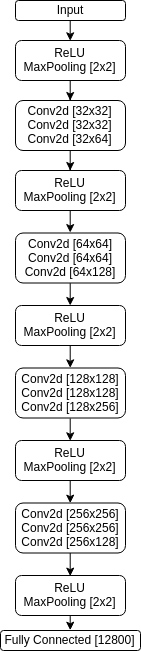
\includegraphics[width=6em]{improved_net.png}
  \caption{Improved ConvNet with 4 Conv2ds blocks followed by ReLU and MaxPooling with final layer being fully connected.}
  \label{fig:improved_conv}
\end{figure}

Our improved model began with a 3x3 convolution on the input data with 3 input channels and 32 output channels. The output of this layer was put into a ReLU layer, followed by a 2x2 max pooling layer. Each block following the input layer is composed of three 3x3 convolution layers, a ReLU activation layer, and a 2x2 max pooling layer. The first two convolutions of these layers take the same number of inputs and outputs to maintain the number of parameters while decreasing the spatial field. The final layer was put through a fully connected layer, taking in 12,800 input features with a single output feature (the probability of cancer being present in the image). This network can be visualized in Fig. \ref{fig:improved_conv}. Our optimal model ended up being 6 layers deep and was able to run on CADE machines without any shortage of memory.


\section{Experiments}
\subsection{Hyper-parameters, Optimizers, and Loss Functions}
Throughout our project, we tried various hyper-parameters and loss functions. Our hyper-parameters consisted of learning rates, batch sizes, and the number of epochs. Details on these hyper-parameters are discussed below along with the loss functions and optimizers:

\subsubsection{Learning Rates}
To determine a proper learning rate for our models, we initially started with wide range of learning rates, $[10, 1, 0.1, 0.01, 0.001, 0.0001]$. After running all of our models on these learning rates, we found that learning rates of $0.01$ to $0.0001$ worked the best for each model. To hone in on the best hyperparameters, we chose three random learning rates between $0.01$ to $0.0001$ (inclusive). We used these learning rates for our models during training. 

\subsubsection{Batch Sizes}
We started to run all of our models on batch sizes from $2$ to $32$ with base $2$ step sizes. As we made test runs, we realized that the ResNet model favored larger batch sizes while the simple and the improved ConvNet models both work well with medium size batches ($8$ or $16$). 

\subsubsection{Epochs}
All of the papers we read used a high amount of epochs with the highest being $3,000$ epochs. Keeping this in mind, we started to train all our models for $50$ epochs to see where the loss rate and the prediction probability would converge. After running all of our models overnight at the CADE lab, almost all of the models converged before $20th$ epoch. In order to save time, we set $20$ as our max epochs for all of our models. 

\subsubsection{Loss Functions}
Initially, we started with Cross Entropy (CE loss). We quickly realized this loss function would take a really long time to converge. The starting loss was very high with cross entropy and the prediction probability was very low. After looking through the PyTorch library, we found Mean Square Error (MSE) loss to give better result for regression problem. Thus we chose MSE loss for our models. MSE loss also converged faster than CE loss which saved us some time in training our models. 

One detail to add here is that with Cross Entropy, we used Cross Entropy with Logits. With MSE loss, we added an additional Softmax layer to the output to make sure the predicted value were from $0$ to $1$. 

\subsubsection{Optimizer}
Throughout the assignments during the semester, we worked with various optimizers. The two popular ones were Sub-gradient Descent (SGD) combined with  momentum and Adam. We tried both of these optimizers on all of our models. However, for our own custom model, the Adam optimizer did not work as well, so we decided to run SGD instead. We chose $0.9$ for the momentum for our SGD optimizer. We tried couple other values for momentum and found $0.9$ to be the best one for this dataset.

\subsection{Results}

\subsubsection{Training ResNet with SGD + Momentum Optimizer}
\begin{figure}[h]
  \centering
  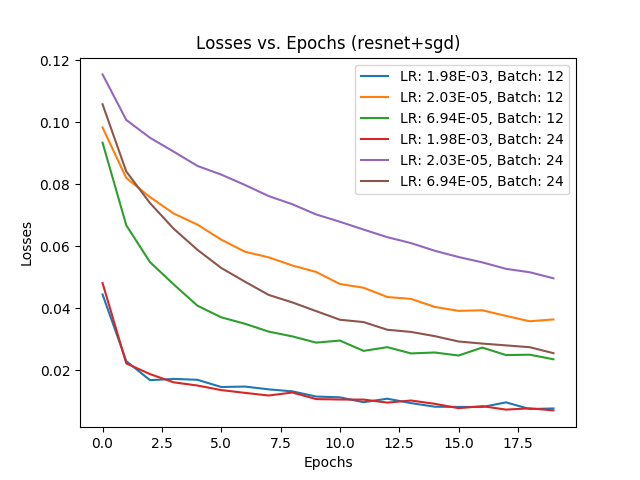
\includegraphics[width=20em]{resnet_sgd_Losses_20e.png}
  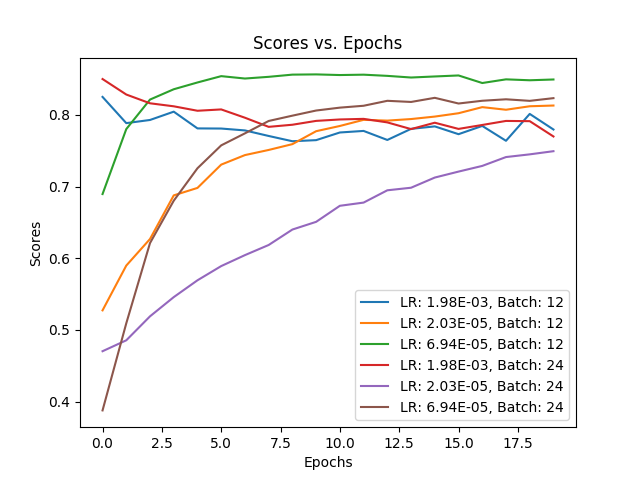
\includegraphics[width=20em]{resnet_sgd_Scores_20e.png}
  \caption{Loss and score results of the ResNet model with various learning rates and batch sizes for 20 epochs.}
  \label{fig:resnet}
\end{figure}

Our final ResNet model  used learning rates of $1.98^{-3}$, $2.03^{-5}$, $6.94^{-5}$, which were found to be the best learning rates. The learning rates were found with randomization between $0.01$ and $0.00001$, inclusive. Our ResNet model also worked best with slightly bigger batch sizes of $12$ and $24$ with an SGD + Momentum optimizer.
With this set up, we found that the model’s best probability prediction on validation dataset was $84.19\%$ during training with a learning rate of $6.94^{-5}$ and a batch size of $24$. The lowest loss was found to be $9.58\%$ with learning rate $1.98^{-3}$ and both batch sizes of $12$ \& $24$.

\subsubsection{Training Initial ConvNet with Adam Optimizer}
\begin{figure}[h]
  \centering
  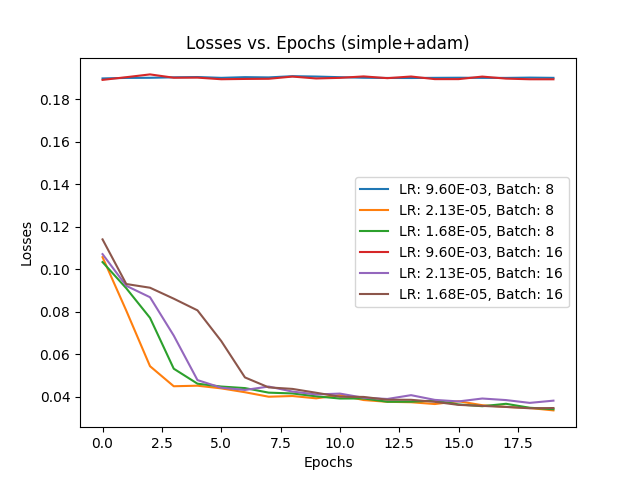
\includegraphics[width=20em]{simple_adam_Losses_20e.png}
  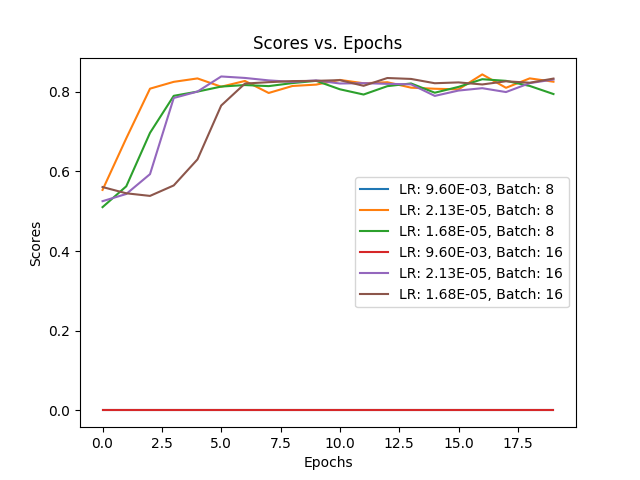
\includegraphics[width=20em]{simple_adam_Scores_20e.png}
  \caption{Loss and score results of the initial ConvNet with Adam optimizer.}
  \label{fig:simple_adam}
\end{figure}

Our initial ConvNet had learning rates of $9.60^{-3}$, $2.13{^-5}$, and $1.68^{-5}$.  This model worked best with smaller batch sizes of $8$ and $16$. Adam optimizer was used during this training run. The best prediction probability made during training for this model was $81.34\%$. As you can see in Fig. \ref{fig:simple_adam}, our initial model did not work well with larger learning rates. Both our loss and prediction probability was unchanged throughout the $20$ epochs.

\subsubsection{Training Initial ConvNet with SGD + Momentum Optimizer}
\begin{figure}[h]
  \centering
  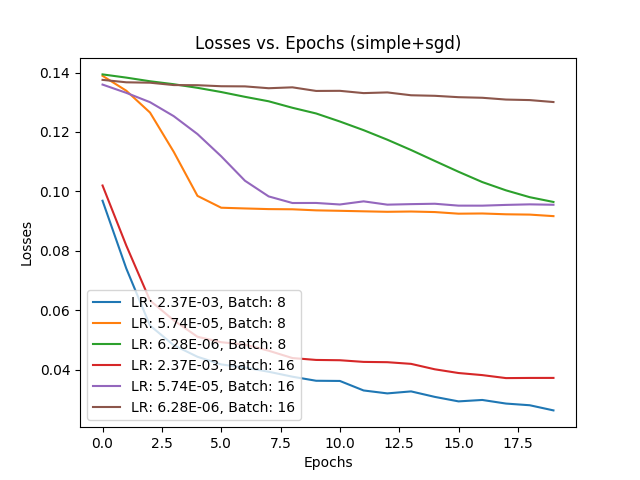
\includegraphics[width=20em]{simple_sgd_Losses_20e.png}
  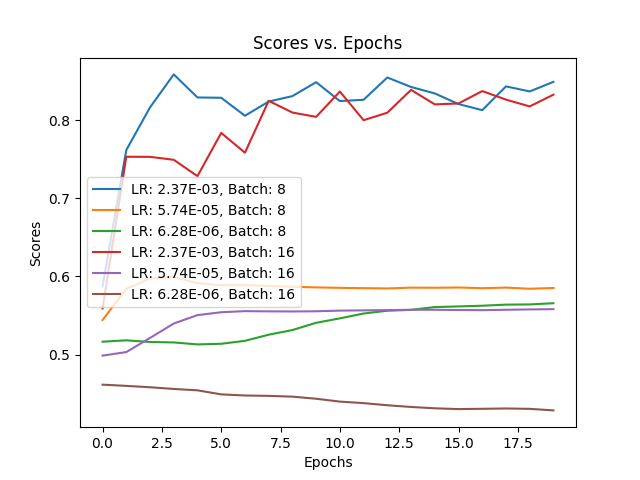
\includegraphics[width=20em]{simple_sgd_Scores_20e.png}
  \caption{Loss and score results of the inital ConvNet with SGD + Momentum optimizer.}
  \label{fig:simple_sgd}
\end{figure}

We also wanted to see how well the same ConvNet would perform with SGD + Momentum optimizer. This time, our best learning rates were $2.37^{-3}$, $5.74^{-5}$, and $6.2^{-6}$. We kept the batch sizes the same from previous training run, i.e. ${8}$ and ${16}$. The best prediction probability achieved during this training was $83.4\%$. With SGD + Momentum, we did notice that the larger learning rates were changing and actually giving the best results as seen in Fig. \ref{fig:simple_sgd}. Since this model showed to have some promise, we expanded on it to see if we could improve the prediction probability.

\subsubsection{Training Improved ConvNet with SGD + Momentum Optimizer}
\begin{figure}[h]
  \centering
  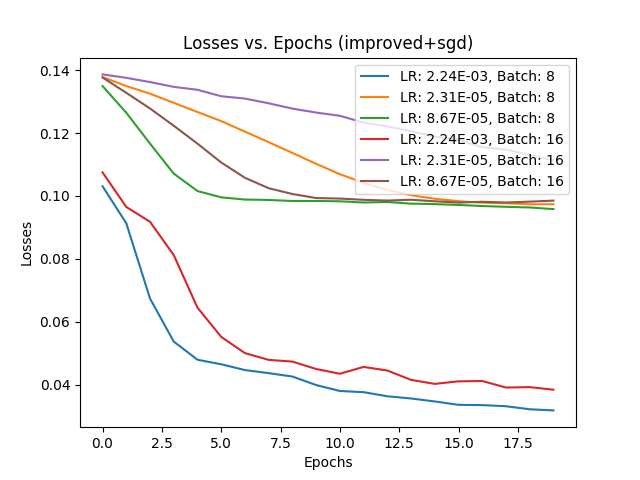
\includegraphics[width=20em]{improved_sgd_Losses_20e.png}
  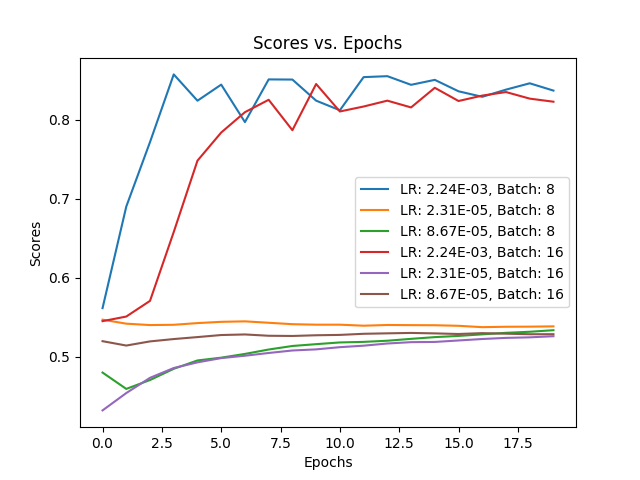
\includegraphics[width=20em]{improved_sgd_Scores_20e.png}
  \caption{Loss and score results of the improved ConvNet with SGD + Momentum optimizer.}
  \label{fig:improved}
\end{figure}

With the improved/modified model, we saw a slight increase in probability prediction during training with the highest probability reaching $85.6\%$. This was made with a learning rate of $2.24^{-3}$ and a batch size of $8$. For the improved ConvNet, we found the SGD + Momentum optimizer to work the best. More detailed loss and score curve can be seen in Fig. \ref{fig:improved}.

\subsubsection{Testing}
Once our networks were trained, we choose the best models mentioned above for each architecture. We found test probabilities for the ResNet, initial ConvNet, and modified ConvNet to be $83.41\%$, $80.13\%$, and $81.37\%$ respectively.

\subsection{Pitfalls}
\subsubsection{GPU memory bottleneck}
During our training with deeper models, we quickly ran into memory issues. To get around this, we tried shallower models and smaller batch sizes. After conducting a few test runs, we realized that deeper models with smaller batch sizes would take longer but had better results. However, to save time we tried shallower models with larger batch sizes which gave us similar results to deeper models. VGG model in particular would not run with our dataset. Thus, we took the ideas of the VGG model and modified it to work with our dataset.

\subsubsection{Adopting classification model for regressoin}
Initially, we wanted to see how well pretrained networks worked. Thus we started with ResNet and VGG. However, since the BreastPathQ is a regression problem, we needed to modify these architectures. It took us some time researching to figure out what would work the best with regression and how we could modify the pretrained classification models.

\subsubsection{Bugs in our framework}
There were many bugs in our framework. The biggest one that we couldn’t catch for a while was model initialization. Our framework creates new models based on user parameters. However, we were not reinitializing our model for every hyper-parameter we trained on. This resulted in inconsistent prediction probabilities and losses. It took us many hours to figure out this simple bug but once we had fixed, it our model began to train as expected.

\subsubsection{Metrics}
We struggled for quite some time when trying to figure out what kind of metrics to use with the data set. As mentioned before, the Spie Challenge website went offline before we were able to start testing our models. We didn’t have access to the site to determine what metrics to use. We experimented with AUC scores, accuracies, etc., but to no success. We eventually found out how to access the cached site from our browser and were able to get access to the provided metrics for the challenge.

\section{Conclusion}
Overall we think this project has helped us understand how the architecture of the networks effects the learning for the dataset. We also learned that understanding the dataset also helps greatly in creating an efficient architecture. 

The next thing we planned on doing with this project was data augmentation. However, with the time constraint, we had to leave this out during the training. We wanted to compare a network trained on vanila images with a network trained on augmented images to see how much data augmentation can change the results of our models. 

We believe that we had successful models, though they do not perform as well as the state of the art models used in practice. With more memory resources, our models could have handled more parameters and deeper networks. Our models could further be improved with more resources. We found the Spie Challenge to be fairly challenging and a great learning experience.

\nocite{*}
\bibliographystyle{IEEEtran}
\bibliography{IEEEabrv,bib/ref.bib}
\end{document}

